
%% bare_conf.tex
%% V1.3
%% 2007/01/11
%% by Michael Shell
%% See:
%% http://www.michaelshell.org/
%% for current contact information.
%%
%% This is a skeleton file demonstrating the use of IEEEtran.cls
%% (requires IEEEtran.cls version 1.7 or later) with an IEEE conference paper.
%%
%% Support sites:
%% http://www.michaelshell.org/tex/ieeetran/
%% http://www.ctan.org/tex-archive/macros/latex/contrib/IEEEtran/
%% and
%% http://www.ieee.org/

%%*************************************************************************
%% Legal Notice:
%% This code is offered as-is without any warranty either expressed or
%% implied; without even the implied warranty of MERCHANTABILITY or
%% FITNESS FOR A PARTICULAR PURPOSE! 
%% User assumes all risk.
%% In no event shall IEEE or any contributor to this code be liable for
%% any damages or losses, including, but not limited to, incidental,
%% consequential, or any other damages, resulting from the use or misuse
%% of any information contained here.
%%
%% All comments are the opinions of their respective authors and are not
%% necessarily endorsed by the IEEE.
%%
%% This work is distributed under the LaTeX Project Public License (LPPL)
%% ( http://www.latex-project.org/ ) version 1.3, and may be freely used,
%% distributed and modified. A copy of the LPPL, version 1.3, is included
%% in the base LaTeX documentation of all distributions of LaTeX released
%% 2003/12/01 or later.
%% Retain all contribution notices and credits.
%% ** Modified files should be clearly indicated as such, including  **
%% ** renaming them and changing author support contact information. **
%%
%% File list of work: IEEEtran.cls, IEEEtran_HOWTO.pdf, bare_adv.tex,
%%                    bare_conf.tex, bare_jrnl.tex, bare_jrnl_compsoc.tex
%%*************************************************************************

% *** Authors should verify (and, if needed, correct) their LaTeX system  ***
% *** with the testflow diagnostic prior to trusting their LaTeX platform ***
% *** with production work. IEEE's font choices can trigger bugs that do  ***
% *** not appear when using other class files.                            ***
% The testflow support page is at:
% http://www.michaelshell.org/tex/testflow/



% Note that the a4paper option is mainly intended so that authors in
% countries using A4 can easily print to A4 and see how their papers will
% look in print - the typesetting of the document will not typically be
% affected with changes in paper size (but the bottom and side margins will).
% Use the testflow package mentioned above to verify correct handling of
% both paper sizes by the user's LaTeX system.
%
% Also note that the "draftcls" or "draftclsnofoot", not "draft", option
% should be used if it is desired that the figures are to be displayed in
% draft mode.
%
\documentclass[conference]{IEEEtran}
% Add the compsoc option for Computer Society conferences.
%
% If IEEEtran.cls has not been installed into the LaTeX system files,
% manually specify the path to it like:
% \documentclass[conference]{../sty/IEEEtran}





% Some very useful LaTeX packages include:
% (uncomment the ones you want to load)


% *** MISC UTILITY PACKAGES ***
%
%\usepackage{ifpdf}
% Heiko Oberdiek's ifpdf.sty is very useful if you need conditional
% compilation based on whether the output is pdf or dvi.
% usage:
% \ifpdf
%   % pdf code
% \else
%   % dvi code
% \fi
% The latest version of ifpdf.sty can be obtained from:
% http://www.ctan.org/tex-archive/macros/latex/contrib/oberdiek/
% Also, note that IEEEtran.cls V1.7 and later provides a builtin
% \ifCLASSINFOpdf conditional that works the same way.
% When switching from latex to pdflatex and vice-versa, the compiler may
% have to be run twice to clear warning/error messages.






% *** CITATION PACKAGES ***
%
%\usepackage{cite}
% cite.sty was written by Donald Arseneau
% V1.6 and later of IEEEtran pre-defines the format of the cite.sty package
% \cite{} output to follow that of IEEE. Loading the cite package will
% result in citation numbers being automatically sorted and properly
% "compressed/ranged". e.g., [1], [9], [2], [7], [5], [6] without using
% cite.sty will become [1], [2], [5]--[7], [9] using cite.sty. cite.sty's
% \cite will automatically add leading space, if needed. Use cite.sty's
% noadjust option (cite.sty V3.8 and later) if you want to turn this off.
% cite.sty is already installed on most LaTeX systems. Be sure and use
% version 4.0 (2003-05-27) and later if using hyperref.sty. cite.sty does
% not currently provide for hyperlinked citations.
% The latest version can be obtained at:
% http://www.ctan.org/tex-archive/macros/latex/contrib/cite/
% The documentation is contained in the cite.sty file itself.


% *** GRAPHICS RELATED PACKAGES ***
%
\ifCLASSINFOpdf
  \usepackage[pdftex]{graphicx}
  % declare the path(s) where your graphic files are
  \graphicspath{{pdf/}{jpeg/}}
  % and their extensions so you won't have to specify these with
  % every instance of \includegraphics
  \DeclareGraphicsExtensions{.pdf,.jpeg,.png}
\else
  % or other class option (dvipsone, dvipdf, if not using dvips). graphicx
  % will default to the driver specified in the system graphics.cfg if no
  % driver is specified.
  \usepackage[dvips]{graphicx}
  % declare the path(s) where your graphic files are
  \graphicspath{{eps/}}
  % and their extensions so you won't have to specify these with
  % every instance of \includegraphics
  \DeclareGraphicsExtensions{.eps}
\fi
% graphicx was written by David Carlisle and Sebastian Rahtz. It is
% required if you want graphics, photos, etc. graphicx.sty is already
% installed on most LaTeX systems. The latest version and documentation can
% be obtained at: 
% http://www.ctan.org/tex-archive/macros/latex/required/graphics/
% Another good source of documentation is "Using Imported Graphics in
% LaTeX2e" by Keith Reckdahl which can be found as epslatex.ps or
% epslatex.pdf at: http://www.ctan.org/tex-archive/info/
%
% latex, and pdflatex in dvi mode, support graphics in encapsulated
% postscript (.eps) format. pdflatex in pdf mode supports graphics
% in .pdf, .jpeg, .png and .mps (metapost) formats. Users should ensure
% that all non-photo figures use a vector format (.eps, .pdf, .mps) and
% not a bitmapped formats (.jpeg, .png). IEEE frowns on bitmapped formats
% which can result in "jaggedy"/blurry rendering of lines and letters as
% well as large increases in file sizes.
%
% You can find documentation about the pdfTeX application at:
% http://www.tug.org/applications/pdftex





% *** MATH PACKAGES ***
%
%\usepackage[cmex10]{amsmath}
% A popular package from the American Mathematical Society that provides
% many useful and powerful commands for dealing with mathematics. If using
% it, be sure to load this package with the cmex10 option to ensure that
% only type 1 fonts will utilized at all point sizes. Without this option,
% it is possible that some math symbols, particularly those within
% footnotes, will be rendered in bitmap form which will result in a
% document that can not be IEEE Xplore compliant!
%
% Also, note that the amsmath package sets \interdisplaylinepenalty to 10000
% thus preventing page breaks from occurring within multiline equations. Use:
%\interdisplaylinepenalty=2500
% after loading amsmath to restore such page breaks as IEEEtran.cls normally
% does. amsmath.sty is already installed on most LaTeX systems. The latest
% version and documentation can be obtained at:
% http://www.ctan.org/tex-archive/macros/latex/required/amslatex/math/





% *** SPECIALIZED LIST PACKAGES ***
%
%\usepackage{algorithmic}
% algorithmic.sty was written by Peter Williams and Rogerio Brito.
% This package provides an algorithmic environment fo describing algorithms.
% You can use the algorithmic environment in-text or within a figure
% environment to provide for a floating algorithm. Do NOT use the algorithm
% floating environment provided by algorithm.sty (by the same authors) or
% algorithm2e.sty (by Christophe Fiorio) as IEEE does not use dedicated
% algorithm float types and packages that provide these will not provide
% correct IEEE style captions. The latest version and documentation of
% algorithmic.sty can be obtained at:
% http://www.ctan.org/tex-archive/macros/latex/contrib/algorithms/
% There is also a support site at:
% http://algorithms.berlios.de/index.html
% Also of interest may be the (relatively newer and more customizable)
% algorithmicx.sty package by Szasz Janos:
% http://www.ctan.org/tex-archive/macros/latex/contrib/algorithmicx/




% *** ALIGNMENT PACKAGES ***
%
%\usepackage{array}
% Frank Mittelbach's and David Carlisle's array.sty patches and improves
% the standard LaTeX2e array and tabular environments to provide better
% appearance and additional user controls. As the default LaTeX2e table
% generation code is lacking to the point of almost being broken with
% respect to the quality of the end results, all users are strongly
% advised to use an enhanced (at the very least that provided by array.sty)
% set of table tools. array.sty is already installed on most systems. The
% latest version and documentation can be obtained at:
% http://www.ctan.org/tex-archive/macros/latex/required/tools/


%\usepackage{mdwmath}
%\usepackage{mdwtab}
% Also highly recommended is Mark Wooding's extremely powerful MDW tools,
% especially mdwmath.sty and mdwtab.sty which are used to format equations
% and tables, respectively. The MDWtools set is already installed on most
% LaTeX systems. The lastest version and documentation is available at:
% http://www.ctan.org/tex-archive/macros/latex/contrib/mdwtools/


% IEEEtran contains the IEEEeqnarray family of commands that can be used to
% generate multiline equations as well as matrices, tables, etc., of high
% quality.


%\usepackage{eqparbox}
% Also of notable interest is Scott Pakin's eqparbox package for creating
% (automatically sized) equal width boxes - aka "natural width parboxes".
% Available at:
% http://www.ctan.org/tex-archive/macros/latex/contrib/eqparbox/





% *** SUBFIGURE PACKAGES ***
%\usepackage[tight,footnotesize]{subfigure}
% subfigure.sty was written by Steven Douglas Cochran. This package makes it
% easy to put subfigures in your figures. e.g., "Figure 1a and 1b". For IEEE
% work, it is a good idea to load it with the tight package option to reduce
% the amount of white space around the subfigures. subfigure.sty is already
% installed on most LaTeX systems. The latest version and documentation can
% be obtained at:
% http://www.ctan.org/tex-archive/obsolete/macros/latex/contrib/subfigure/
% subfigure.sty has been superceeded by subfig.sty.



%\usepackage[caption=false]{caption}
\usepackage[font=footnotesize]{subfig}
% subfig.sty, also written by Steven Douglas Cochran, is the modern
% replacement for subfigure.sty. However, subfig.sty requires and
% automatically loads Axel Sommerfeldt's caption.sty which will override
% IEEEtran.cls handling of captions and this will result in nonIEEE style
% figure/table captions. To prevent this problem, be sure and preload
% caption.sty with its "caption=false" package option. This is will preserve
% IEEEtran.cls handing of captions. Version 1.3 (2005/06/28) and later 
% (recommended due to many improvements over 1.2) of subfig.sty supports
% the caption=false option directly:
%\usepackage[caption=false,font=footnotesize]{subfig}
%
% The latest version and documentation can be obtained at:
% http://www.ctan.org/tex-archive/macros/latex/contrib/subfig/
% The latest version and documentation of caption.sty can be obtained at:
% http://www.ctan.org/tex-archive/macros/latex/contrib/caption/




% *** FLOAT PACKAGES ***
%
%\usepackage{fixltx2e}
% fixltx2e, the successor to the earlier fix2col.sty, was written by
% Frank Mittelbach and David Carlisle. This package corrects a few problems
% in the LaTeX2e kernel, the most notable of which is that in current
% LaTeX2e releases, the ordering of single and double column floats is not
% guaranteed to be preserved. Thus, an unpatched LaTeX2e can allow a
% single column figure to be placed prior to an earlier double column
% figure. The latest version and documentation can be found at:
% http://www.ctan.org/tex-archive/macros/latex/base/



%\usepackage{stfloats}
% stfloats.sty was written by Sigitas Tolusis. This package gives LaTeX2e
% the ability to do double column floats at the bottom of the page as well
% as the top. (e.g., "\begin{figure*}[!b]" is not normally possible in
% LaTeX2e). It also provides a command:
%\fnbelowfloat
% to enable the placement of footnotes below bottom floats (the standard
% LaTeX2e kernel puts them above bottom floats). This is an invasive package
% which rewrites many portions of the LaTeX2e float routines. It may not work
% with other packages that modify the LaTeX2e float routines. The latest
% version and documentation can be obtained at:
% http://www.ctan.org/tex-archive/macros/latex/contrib/sttools/
% Documentation is contained in the stfloats.sty comments as well as in the
% presfull.pdf file. Do not use the stfloats baselinefloat ability as IEEE
% does not allow \baselineskip to stretch. Authors submitting work to the
% IEEE should note that IEEE rarely uses double column equations and
% that authors should try to avoid such use. Do not be tempted to use the
% cuted.sty or midfloat.sty packages (also by Sigitas Tolusis) as IEEE does
% not format its papers in such ways.





% *** PDF, URL AND HYPERLINK PACKAGES ***
%
%\usepackage{url}
% url.sty was written by Donald Arseneau. It provides better support for
% handling and breaking URLs. url.sty is already installed on most LaTeX
% systems. The latest version can be obtained at:
% http://www.ctan.org/tex-archive/macros/latex/contrib/misc/
% Read the url.sty source comments for usage information. Basically,
% \url{my_url_here}.





% *** Do not adjust lengths that control margins, column widths, etc. ***
% *** Do not use packages that alter fonts (such as pslatex).         ***
% There should be no need to do such things with IEEEtran.cls V1.6 and later.
% (Unless specifically asked to do so by the journal or conference you plan
% to submit to, of course. )


% correct bad hyphenation here
\hyphenation{op-tical net-works semi-conduc-tor}


\begin{document}
%
% paper title
% can use linebreaks \\ within to get better formatting as desired
\title{A Virtual Cluster Manager using a Hierarchical Management Model for Cloud Infrastructure}


% author names and affiliations
% use a multiple column layout for up to three different
% affiliations
%\author{\IEEEauthorblockN{Pongsakorn U-chupala}
%\IEEEauthorblockA{Faculty of Computer Engineering\\
%Kasetsart University, Bangkok, Thailand\\
%Email: b5105274@ku.ac.th}}

% conference papers do not typically use \thanks and this command
% is locked out in conference mode. If really needed, such as for
% the acknowledgment of grants, issue a \IEEEoverridecommandlockouts
% after \documentclass

% for over three affiliations, or if they all won't fit within the width
% of the page, use this alternative format:
% 
\author{\IEEEauthorblockN{Pongsakorn U-chupala\IEEEauthorrefmark{1},
Kohei Ichikawa\IEEEauthorrefmark{2},
Hirotake Abe, 
Susumu Date and
Shinji Shimojo\IEEEauthorrefmark{3}}
\IEEEauthorblockA{\IEEEauthorrefmark{1}Department of Computer Engineering, 
Kasetsart University, Bangkok, Thailand\\
Email: b5105274@ku.ac.th}
\IEEEauthorblockA{\IEEEauthorrefmark{2}Central Office for Information Infrastructure, 
Osaka University, Osaka, Japan\\
Email: ichikawa@cmc.osaka-u.ac.jp}
\IEEEauthorblockA{\IEEEauthorrefmark{3}Cybermedia Center, 
Osaka University, Osaka, Japan\\
Email: \{habe, date, shimojo\}@cmc.osaka-u.ac.jp}
}




% use for special paper notices
%\IEEEspecialpapernotice{(Invited Paper)}




% make the title area
\maketitle


\begin{abstract}
%\boldmath
With cloud computing technology, specifically infrastructure as a service (IaaS), it is possible to conveniently deploy a virtual machine on the cloud.
There are also a lot of cloud toolkits available to help administrators setup IaaS cloud.
However, to deploy a set of virtual machines and configure them to work together as a virtual cluster is still a complicated and tedious task.
Most cloud toolkits offer not comprehensive virtual cluster management solution but individual virtual machine management.
To address this problem, we propose virtual cluster manager, a unified utility for virtual cluster management.
This paper describes a design and implementation of virtual cluster manager built on top of existing cloud toolkit, OpenNebula, as well as the case study of this utility through the comparison with virtual cluster deployment with traditional methods.
\end{abstract}
% IEEEtran.cls defaults to using nonbold math in the Abstract.
% This preserves the distinction between vectors and scalars. However,
% if the conference you are submitting to favors bold math in the abstract,
% then you can use LaTeX's standard command \boldmath at the very start
% of the abstract to achieve this. Many IEEE journals/conferences frown on
% math in the abstract anyway.

%\begin{IEEEkeywords}
%Cloud Computing; Virtual Cluster; Virtual Infrastructure;
%
%\end{IEEEkeywords}



% For peer review papers, you can put extra information on the cover
% page as needed:
% \ifCLASSOPTIONpeerreview
% \begin{center} \bfseries EDICS Category: 3-BBND \end{center}
% \fi
%
% For peerreview papers, this IEEEtran command inserts a page break and
% creates the second title. It will be ignored for other modes.
\IEEEpeerreviewmaketitle



\section{Introduction}
% no \IEEEPARstart
%This demo file is intended to serve as a ``starter file''
%for IEEE conference papers produced under \LaTeX\ using
%IEEEtran.cls version 1.7 and later.
% You must have at least 2 lines in the paragraph with the drop letter
% (should never be an issue)
%I wish you the best of success.
%\hfill mds 
%\hfill January 11, 2007
With cloud computing \cite{Armbrust:EECS-2009-28} being a buzzword recently, there are a wide range of cloud computing toolkits available nowadays.
Each provides services in different abstraction.
In this research, we focus on Infrastructure as a Service (IaaS) \cite{ranabahu2009best} paradigm.
These toolkits offer the ability to manage resources ubiquitously with united cloud interface.

Even though virtual infrastructure (VI) provides virtually limitless computation capability to user, in reality, performance of each virtual machine (VM) running on the infrastructure is still limited by physical host machine.
It turned out that we have already solved this problem with cluster computing.
We could use this same methodology and create a cluster of VM instead of physical machine.
This technology is called Virtual Cluster (VC) \cite{1630864}.

However, most VI toolkits (such as OpenNebula \cite{10.1109/MIC.2009.119} and Eucalyptus \cite{nurmi2009eucalyptus}) only focus on individual VM management.
Although it allows us to build VC with these existing toolkits by configuring and deploying each VM manually, there is no convenient way to manage VC as a whole yet.
To simplify this process, we propose a utility that manages VC with existing VI toolkit.
This utility will provide users another layer of abstraction that allows users to view the system as a repository for VC.

In this research, we have developed CLI Utility called \emph{onevc} for OpenNebula 3.0 (VI toolkit) which provides the ability to manage VC as a whole.
This utility works alongside other built-in CLI utilities seamlessly and provides interface similar to existing built-in utilities for consistency.

This paper is structured as follows.
Section II describes OpenNebula in general, similar utility called ``oneservice'' and differences between ``oneservice'' and this research.
Section III describes the architecture of VC manager.
Section IV describes VC manager implementation based on OpenNebula VI toolkit.
Section V demonstrates cases where VC manager performs better than existing utilities and their measurement.
Section VI is the conclusion and future directions.

%\subsection{Subsection Heading Here}
%Subsection text here.
%\subsubsection{Subsubsection Heading Here}
%Subsubsection text here.


% An example of a floating figure using the graphicx package.
% Note that \label must occur AFTER (or within) \caption.
% For figures, \caption should occur after the \includegraphics.
% Note that IEEEtran v1.7 and later has special internal code that
% is designed to preserve the operation of \label within \caption
% even when the captionsoff option is in effect. However, because
% of issues like this, it may be the safest practice to put all your
% \label just after \caption rather than within \caption{}.
%
% Reminder: the "draftcls" or "draftclsnofoot", not "draft", class
% option should be used if it is desired that the figures are to be
% displayed while in draft mode.
%

% Note that IEEE typically puts floats only at the top, even when this
% results in a large percentage of a column being occupied by floats.


% An example of a double column floating figure using two subfigures.
% (The subfig.sty package must be loaded for this to work.)
% The subfigure \label commands are set within each subfloat command, the
% \label for the overall figure must come after \caption.
% \hfil must be used as a separator to get equal spacing.
% The subfigure.sty package works much the same way, except \subfigure is
% used instead of \subfloat.
%
%\begin{figure*}[!t]
%\centerline{\subfloat[Case I]\includegraphics[width=2.5in]{subfigcase1}%
%\label{fig_first_case}}
%\hfil
%\subfloat[Case II]{\includegraphics[width=2.5in]{subfigcase2}%
%\label{fig_second_case}}}
%\caption{Simulation results}
%\label{fig_sim}
%\end{figure*}
%
% Note that often IEEE papers with subfigures do not employ subfigure
% captions (using the optional argument to \subfloat), but instead will
% reference/describe all of them (a), (b), etc., within the main caption.


% An example of a floating table. Note that, for IEEE style tables, the 
% \caption command should come BEFORE the table. Table text will default to
% \footnotesize as IEEE normally uses this smaller font for tables.
% The \label must come after \caption as always.
%
%\begin{table}[!t]
% increase table row spacing, adjust to taste
%\renewcommand{\arraystretch}{1.3}
% if using array.sty, it might be a good idea to tweak the value of
% \extrarowheight as needed to properly center the text within the cells
%\caption{An Example of a Table}
%\label{table_example}
%\centering
%% Some packages, such as MDW tools, offer better commands for making tables
%% than the plain LaTeX2e tabular which is used here.
%\begin{tabular}{|c|c|}
%\hline
%oid & Two\\
%\hline
%name & Four\\
%\hline
%body & Four\\
%\hline
%uid & Four\\
%\hline
%gid & Four\\
%\hline
%last_poll & Four\\
%\hline
%state & Four\\
%\hline
%lcm_state & Four\\
%\hline
%\end{tabular}
%\end{table}


% Note that IEEE does not put floats in the very first column - or typically
% anywhere on the first page for that matter. Also, in-text middle ("here")
% positioning is not used. Most IEEE journals/conferences use top floats
% exclusively. Note that, LaTeX2e, unlike IEEE journals/conferences, places
% footnotes above bottom floats. This can be corrected via the \fnbelowfloat
% command of the stfloats package.

\section{OpenNebula as a Building Block}

\begin{figure}[!t]
\centering
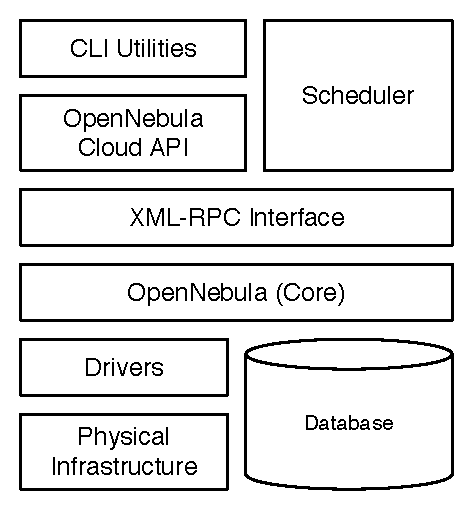
\includegraphics[width=2.2in]{onearch}
\caption{OpenNebula software stack (simplified) \cite{introapis}.}
\label{fig:onearch}
\end{figure}

\begin{figure*}[!t]
\centering
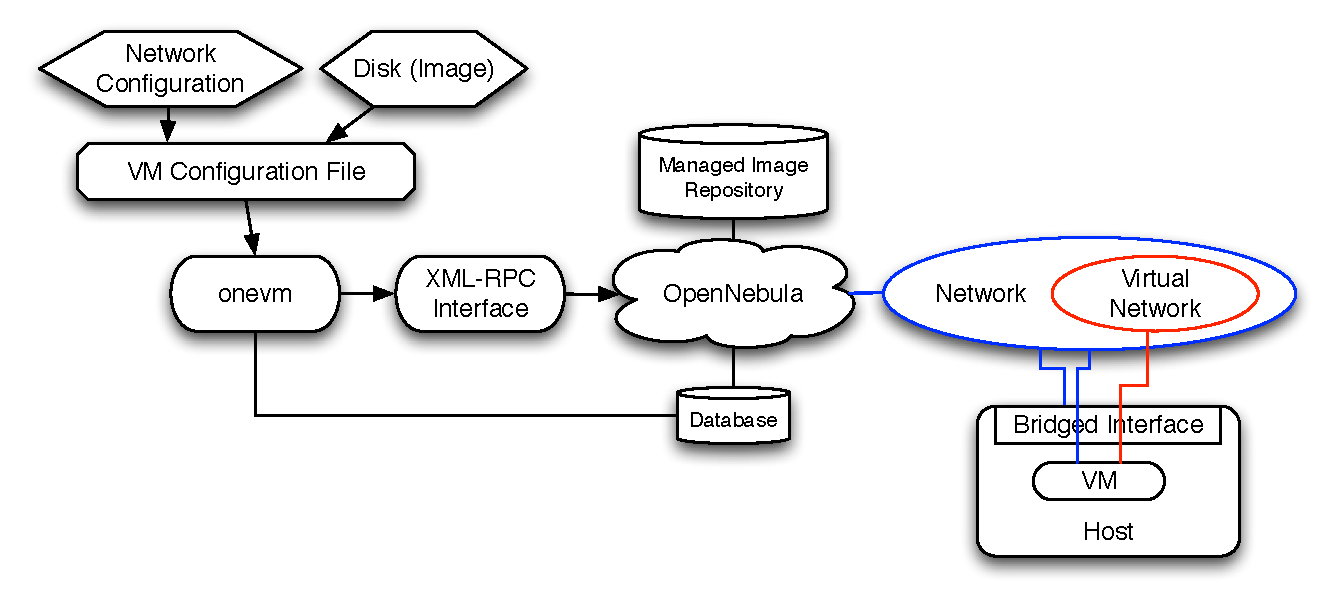
\includegraphics[width=6.5in]{onevm}
\caption{onevm VM deployment process with one deployed VM.}
\label{fig:onevm}
\end{figure*}

\subsection{OpenNebula}
In this paper, we refer to OpenNebula. Thus, it is needed to briefly explain about OpenNebula and its architecture for later discussion.

OpenNebula is a VI manager. It orchestrates VM placement, networking and resources such as disk images and exposes unified cloud interface to its users, thus creates an IaaS cloud.
It enables creation of private cloud with existing resources.
OpenNebula also is characterized with its modular architecture, which allows it to work with several hypervisors.
This feature also enables OpenNebula to support creation of hybrid cloud as well.

To archive a high level of scalability, OpenNebula architecture is designed to be modular.
Using drivers, OpenNebula can be plugged into a wide range of datacenter services.
The software stack is also divided into multiple layers.
This approach allows us to modify and extend OpenNebula as needed.
Figure \ref{fig:onearch} show the architecture of OpenNebula software stack.

To manage the cloud, OpenNebula is shipped with a number of built-in CLI utilities such as \emph{onevm}, \emph{onevnet}, \emph{onehost} and \emph{onetemplate}.
These utilities provide the information of the cloud as well as perform various tasks such as VM deployment and deletion on each subsystem of OpenNebula.
Each utility connects to OpenNebula via OpenNebula Cloud API (OCA) and provides abilities to manage the cloud.
OpenNebula maintains pools of hosts, disk images, network configurations, VM templates and VM instances with \emph{onehost}, \emph{oneimage}, \emph{onevnet}, \emph{onetemplate} and \emph{onevm} respectively.
To register a configuration into each pool, users need to provide a template for each utility accordingly (i.e. supply network configuration template to \emph{onevnet} to add network configuration the pool) with the exception of \emph{onehost} which accepts parameters directly from the shell.
VM template could then refer registered resources (network configurations, disk images, etc.) to be used.

After all configurations are in place, to deploy VM, users need to register VM templates to the template pool and use \emph{onetemplate} utility to instantiate VM instances or just supply the templates to \emph{onevm} utility directly.
Figure \ref{fig:onevm} shows deployment operation flow of \emph{onevm}.

\subsection{oneservice}
There is a concept of service which is consisted of multiple VMs working together being developed for OpenNebula.
For an example a web server service could consists of web servers, database servers and load-balancers.
oneservice \cite{oneservice} utility allow user to describe service and its dependencies with Service Description Language (SDL).
This idea is similar to the virtual cluster but the key difference is service management allows user to manage as group of virtual machines as a whole while virtual cluster management allows user to manage the whole cluster or just a subset of machines in the cluster.

\section{Architecture}
Similar to how \emph{onevm} utility of OpenNebula works, to describe a VC to VC manager, we have adopted hierarchical template system.
This template system allows user to describe VC attributes in one single template file.
This template extends existing VM template system for VC deployment.
VC manager takes VC template as an input and then registers the VC to the database.
After that, users can instruct the manager to do management operations on registered VC or each VM type individually.
Supported management operations are create, deploy, suspend, stop, resume, delete, list and show.

\begin{figure}[!t]
\centering
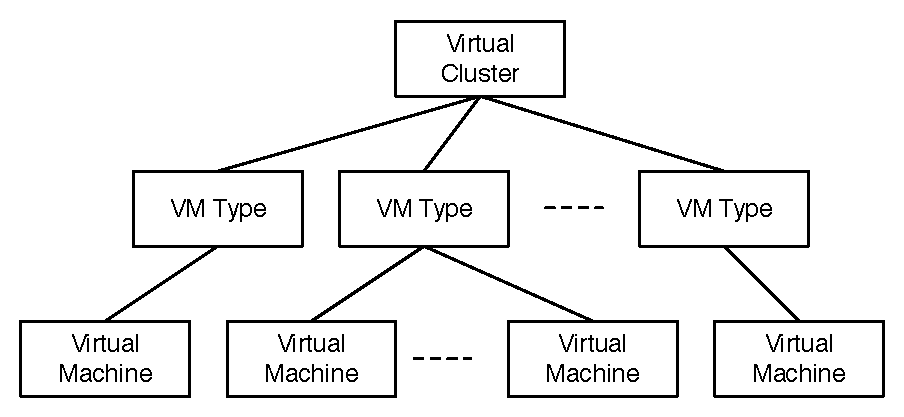
\includegraphics[width=3.5in]{model}
\caption{Hierarchical model of virtual cluster.}
\label{fig:model}
\end{figure}

\subsection{Virtual Cluster Model}
In this research, we have defined VC with a hierarchical model.
A VC consists of one or multiple VM type, served as a grouping method for VM.
A number of VMs could be instantiated in each VM type.
Figure \ref{fig:model} shows hierarchy of VC in this model.

VM types in VC also forms its own hierarchy.
This hierarchy is used along with other configurations to determine the deployment order of each VM in a VC.

One example is a VC with one frontend machine and a number of compute nodes.
To represent this VC with this model, 2 VM types to represent frontend VC and compute node VM are used.
The frontend VM type contains only one VM while the compute nodes VM type contains \emph{n} number of VM with the compute nodes VM type being a child of the frontend VM type.

\begin{figure}[!t]
\centering
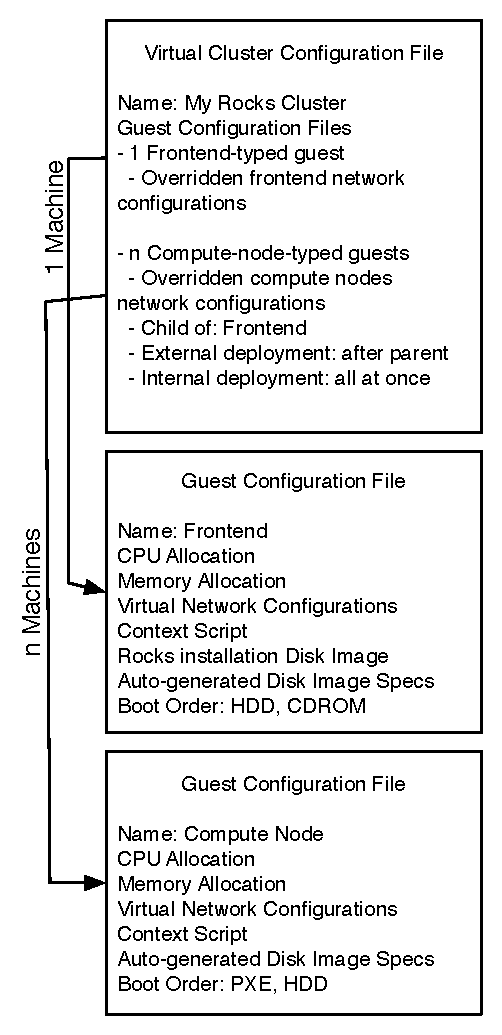
\includegraphics[width=2.5in]{template}
\caption{Example VC template (detail omitted).}
\label{fig:template}
\end{figure}

\begin{figure}[!t]
\centering
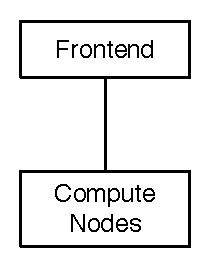
\includegraphics[width=1in]{hierarchy}
\caption{VM type hierarchy of example VC template.}
\label{fig:hierarchy}
\end{figure}

\subsection{Virtual Cluster Template}
To describe a VC with our model, we use template.
For each VC, a VC template is used to describe its properties.
This VC template syntax is the same as OpenNebula template syntax to preserve consistency with others built-in utilities, to be more familiar to user.
VC properties may include information such as name, VC types and number of VM to deploy for each VM type.

To describe each VM type in VC template, we use the same OpenNebula VM template structure.
We also allow pointing to external VM template path or template id of template registered in \emph{onetemplate} built-in utility.
If VC template is defined with either of these 2 methods, we also allow VM type template overriding from VC template as well.
This allows VM type sharing between many VC templates as we could modify VC specific configuration such as networking as needed.

Each VM type is also configurable with external deployment policy such as ``with parent'', ``after parent'' or ``manual'' and internal deployment policy such as ``all together'' or ``one by one''.
These policies will be used to determine deployment order of each VM for automatic cluster deployment.
Figure \ref{fig:template} is shown as an example of cluster VC template.

To determine deployment order, firstly, we use external deployment policy and VM type hierarchy to determine deployment order of VM type.
VM type that does not have parent will be deployed first.
If there are any child VM type of these VM which external deployment policy set to ``with parent'', those VM type will be deployed at the same time.
After all of these VM types successfully deployed (reached ``running'' state), their children will be deployed next, and so on until all VM type is deployed.
For deployment order of each machine in the same VM type, we use internal deployment policy.

\begin{figure}[!t]
\centering
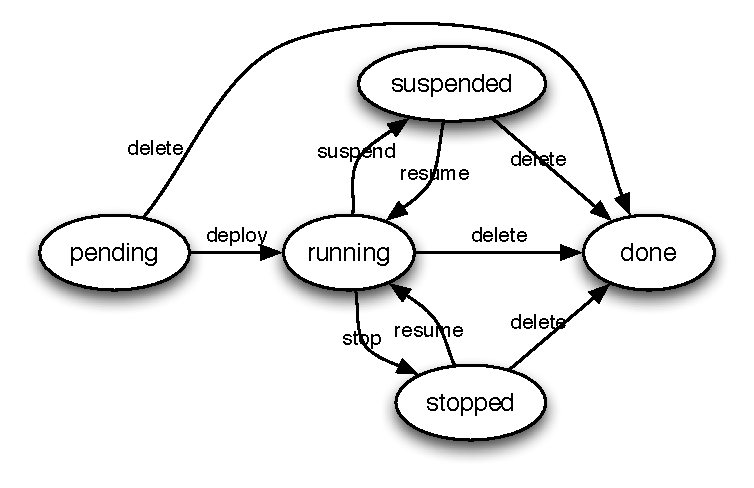
\includegraphics[width=3.5in]{state}
\caption{VC and VM Type state diagram.}
\label{fig:state}
\end{figure}

\begin{figure*}[!t]
\centering
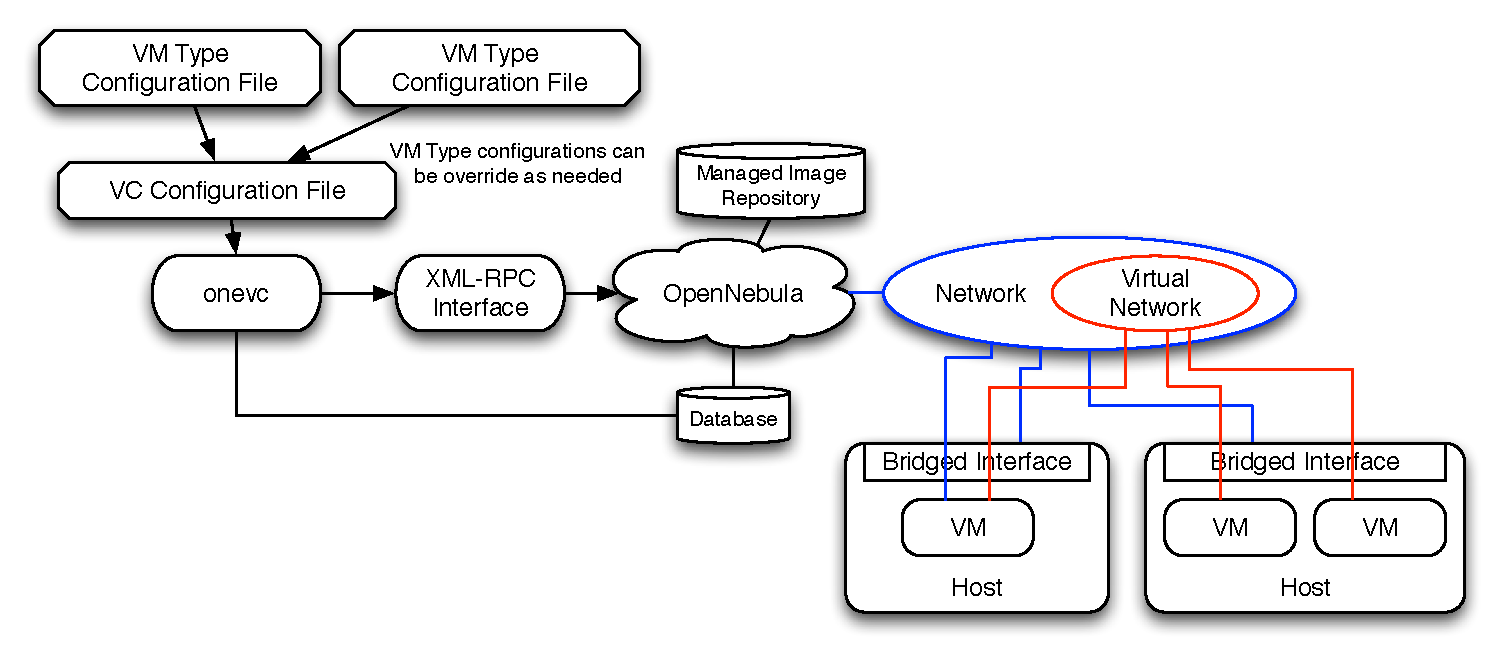
\includegraphics[width=6.5in]{onevc}
\caption{onevc VC deployment process with 1 deployed VC of 3 VM.}
\label{fig:onevc}
\end{figure*}

\subsection{Virtual Cluster State}
We assign state to each VM type in a VC and the VC itself in order to keep tracking.
During initialization, all VM type will be assigned to ``pending'' state.
State of VM type is shifted along with VC management operations (deploy, suspend, resume, etc.).
State shifting is described in Figure \ref{fig:state}.
These states are designed to support OpenNebula's VM state \cite{opennebula-state} and bear a similarity with it.

When all VM type in a VC is in the same state, VC itself is assigned with that state as well.
Otherwise, the VC is assigned ``shift'' intermediate state to indicate that the state is being shifted and currently inconsistent.

\section{Implementation}
VC Manager has been implemented as OpenNebula CLI utility and named \emph{onevc} for consistency with other OpenNebula CLI utilities.
\emph{onevc} is written in Ruby just like other built-in CLI utilities.
It works along with other built-in CLI utilities on the same layer and relied on the same OCA interface.
However, we need to create some more tables in the database to hold VC information.

\subsection{Database}
We use existing mechanism provided by OpenNebula to manage VM so it uses existing \texttt{vm\_pool} table as well.
For VM type, we use existing template system and by storing VM type configuration as template in existing \texttt{template\_pool}.
We define 3 additional tables in the database, \texttt{vc\_pool}, \texttt{vc\_node} and \texttt{vm\_type}.
\texttt{vc\_pool} stores VCs registered to \emph{onevc}, their configuration from their template and their state.
\texttt{vm\_type} associates each VM type specified in VC template with the actual VM type configuration stored in \texttt{template\_pool}.
\texttt{vc\_node} associates each VM with its VC in \texttt{vc\_pool} and VM type in \texttt{template\_pool} as well as recording its state.
Figure \ref{fig:database} shows the relationship between each table.

\begin{figure}[!t]
\centering
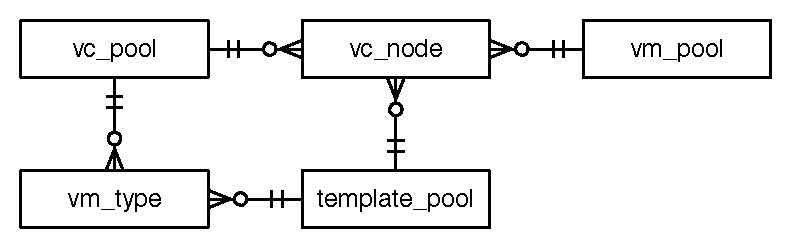
\includegraphics[width=3.5in]{database}
\caption{ER diagram of onevc database.}
\label{fig:database}
\end{figure}

\subsection{Operation}
User can supply VC template to \emph{onevc} in the same fashion as with \emph{onevm} utility.
\emph{onevc} validates the template, puts it into \emph{onevc} \texttt{vc\_pool} table and assign all VM type and the VC itself with ``pending'' state.
After that, \emph{onevc} creates all VC with OpenNebula then puts all of them in OpenNebula's ``pending'' state, waiting for deployment.
Users could then deploy registered VC and do management tasks with \emph{onevc} utility.
Figure \ref{fig:onevc} shows the VC deployment process of \emph{onevc}.

\emph{onevc} utility support the following operations.

\begin{itemize}
\item \texttt{create}\\ register VC template to \emph{onevc} utility and initialize VC
\item \texttt{deploy}\\ deploy specified VC or specified VM type according to VM type hierarchy and deployment policy in VC template 
\item \texttt{suspend}\\ suspend VC or specified VM type in reverse order of deployment
\item \texttt{stop}\\ stop VC or specified VM type in reverse order of deployment
\item \texttt{resume}\\ resume VC or specified VM type in the same order as deployment
\item \texttt{delete}\\ delete VC or specified VM type in reverse order of deployment
\item \texttt{list}\\ list registered VCs and their statuses
\item \texttt{show}\\ show specified VC information
\end{itemize}

\section{Case Study}
To show advantages of our VC manager design, the following cases are considered.
 
\subsection{Ease of use}
We use number of commands used to deploy a VC to demonstrate ease of use of the manager.
The less command needed, the more convenient it is.
Using the example VC template in Figure \ref{fig:template}, we deploy the VC with existing utility and \emph{onevc} utility.

\subsubsection{With existing built-in utility}
Firstly, we created 2 templates for frontend and compute nodes and register it to \emph{onetemplate} built-in utility with this command.

\texttt{\$ onetemplate create <path\_to\_templatefile>}

Then, we instantiate 1 frontend VM followed by a number of compute nodes.
To instantiate VM with \emph{onetemplate}, we used this command.

\texttt{\$ onetemplate instantiate <template\_id>}

Where \texttt{<template\_id>} is template's id given to registered template.
It took two commands to register templates, one command to instantiate frontend and the other to instantiate each compute node, so we used 3+n commands in total.
We also need to maintain each template individually and make sure that configurations in both templates worked together.

\subsubsection{With onevc utility}

Let the name of VC configuration file is \texttt{mycluster.one}, Firstly, user needs to register the template with this command

\texttt{\$ onevc create mycluster.one}

After registration, user can use this command.

\texttt{\$ onevc deploy mycluster}

According to deployment policies in the template, \emph{onevm} will deploy frontend VM first.
After it reach ``running'' state, it will deploy \emph{n} number of compute nodes at once.
User can choose to deploy each VM type manually by using these following commands. 

\texttt{\$ onevc deploy mycluster frontend}

\texttt{\$ onevc deploy mycluster computenodes}

Note that if frontend VM type isn't at ``running'' state when user manually deploy compute nodes then \emph{onevm} will try to move frontend to ``running'' state by deploying or resuming as necessary.

In total, we used 2 commands for automatic deployment and 3 commands for manual VM type deployment regardless of how many compute nodes are there in the cluster.

\subsection{Template Reusability}
With VM type hierarchical structure, it is possible to reuse VM type across multiple VC.
To demonstrate this point, we use number of templates needed as a measurement.
In this case, we will deploy 3 virtual Rocks Clusters \cite{CPE:CPE722} with different number of compute nodes for each VC (\emph{l}, \emph{m} and \emph{n} compute nodes).

\subsubsection{With existing built-in utility}
For each VC, we need 2 VM templates file for frontend node and compute nodes.
Even if some part of frontend node and compute nodes share the same configuration, there are differences between each template (such as network configuration to use) so configuration file need to be duplicated and maintained individually.
In total, 6 VM templates are needed.
Each node also needs to be deployed manually, so OpenNebula cannot keep track of number of compute nodes for each VC at all.
Figure \ref{fig:vmtypeshare} shows VC Hierarchy of these configurations.

\begin{figure}[!t]
\centering
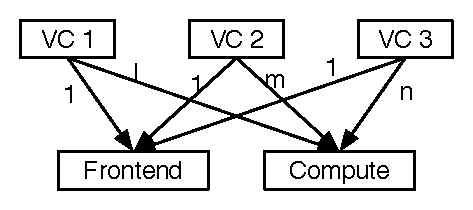
\includegraphics[width=2.5in]{vmtypeshare}
\caption{VM type sharing between multiple VC.}
\label{fig:vmtypeshare}
\end{figure}

\subsubsection{With onevc utility}
Because frontend node and compute nodes for each VC bare similarity, we define them with single VM type template for each one.
Each VC can just point to these 2 VM type template, specify number of compute node needed and override unique configuration for each VC.
We need 3 VC templates and 2 VM type templates so there are 6 templates needed in total.

\section{Conclusion and Future Work}
In this paper, we have described a convenient utility for VC management with existing VI toolkit.
Instead of managing each VM in a VC individually, this utility offers a method for managing VC as a whole.
In order to flexibly describe VC, we use hierarchical VC model along with the template system.
This template system also offers policy configurations to be used alongside VM type hierarchy to determine deployment order.
With this architecture, we have implemented \emph{onevc} utility for OpenNebula and showed how to deploy typical VC with this tool through the comparison with existing built-in utility.
Our case study implies that this VC manager make VC management simpler and convieneint.

However, we only look into VC management and leave VC template management totally to users.
For this issue, we could create another utility to manage VC template.
This utility could work in the same manner as \emph{onetemplate} built-in utility of OpenNebula manage VM template but with VC template instead.

% conference papers do not normally have an appendix


% use section* for acknowledgement
%\newpage
\section*{Acknowledgment}
This research is partly supported by the joint research project titled "Research on structuring method of multiple overlay networks leveraging NGN", between Osaka University and NTT Cyber Solutions Laboratories. Also, this research was partly supported by the Ministry of Education, Culture, Sports, Science and Technology, Grant-in-Aid for Young Scientists (B) [No. 22700052, 23700058].
The authors would like to thank Shimojo Lab for providing research facilities, FrontierLab@OsakaU program for the opportunity and Japan Student Services Organization (JASSO) for their financial support.





% trigger a \newpage just before the given reference
% number - used to balance the columns on the last page
% adjust value as needed - may need to be readjusted if
% the document is modified later
%\IEEEtriggeratref{8}
% The "triggered" command can be changed if desired:
%\IEEEtriggercmd{\enlargethispage{-5in}}

% references section

% can use a bibliography generated by BibTeX as a .bbl file
% BibTeX documentation can be easily obtained at:
% http://www.ctan.org/tex-archive/biblio/bibtex/contrib/doc/
% The IEEEtran BibTeX style support page is at:
% http://www.michaelshell.org/tex/ieeetran/bibtex/
\bibliographystyle{IEEEtran}
% argument is your BibTeX string definitions and bibliography database(s)
\bibliography{IEEEabrv,bibdesk}
%
% <OR> manually copy in the resultant .bbl file
% set second argument of \begin to the number of references
% (used to reserve space for the reference number labels box)
%\begin{thebibliography}{1}
%
%\bibitem{10.1109/MIC.2009.119}
%B.~Sotomayor, R.~S. Montero, I.~M. Llorente, and I.~Foster.
%\newblock Virtual infrastructure management in private and hybrid clouds.
%\newblock {\em IEEE Internet Computing}, 13(5):14--22, 2009.
%
%\bibitem{1630864}
%I.~Foster, T.~Freeman, K.~Keahy, D.~Scheftner, B.~Sotomayer, and X.~Zhang.
%\newblock Virtual clusters for grid communities.
%\newblock In {\em Cluster Computing and the Grid, 2006. CCGRID 06. Sixth IEEE
%  International Symposium on}, volume~1, pages 513 -- 520, {may} 2006.
%
%\end{thebibliography}




% that's all folks
\end{document}


